\documentclass{../tuda-beamer}
\usepackage{wasysym}

% Title information
\authors{Simon Hock}
\authors{Nhan Huynh}
\authors{Daniel Mangold}
\date{08. Dezember 2021}

% Document
\begin{document}

  \maketitle

  \begin{frame}{Überblick}
    \tableofcontents
  \end{frame}


  \section{Organisatorisches}
  \begin{frame}{Organisatorisches}
    \begin{itemize}
      \item 15.12.2021 Präsenzsprechstunde im Raum in Raum S103/\textbf{223}!
    \end{itemize}
  \end{frame}


  \section{Lambda-Ausdrücke}
  \begin{frame}{Lambda-Ausdrücke}
    \begin{itemize}
      \item Anonyme Funktion
      \item Keinen Namen / Bezeichner
    \end{itemize}
  \end{frame}

  \begin{frame}{Lamba-Ausdrücke - Racket}
    \begin{itemize}
      \item Schlüsselwort \inlineracket{lambda} oder \textcolor{keywordcolor}{\(\lambda\)}
      \item Argumente optional, werden mit Leerzeichen getrennt
      \begin{itemize}
        \item Klammer müssen trotzdem notiert werden!
      \end{itemize}
      \item Argumente an Lambda-Ausdruck übergeben: Lambda-Ausdruck wird mit runden Klammern
      umschlossen, in welchen zuerst der Lambda-Ausdruck steht, gefolgt von den Argumenten
    \end{itemize}
    \lstinputlisting[style=Racket, mathescape]{codes/lambda_formal.rkt}
  \end{frame}

  \begin{frame}[c]
    \lstinputlisting[style=Racket, title=Beispiel: Normale Funktion]{codes/add_fct.rkt}
  \end{frame}

  \begin{frame}
    \lstinputlisting[style=Racket, title=Beispiel: Lambda-Ausdruck]{codes/add_lambda_fct.rkt}
  \end{frame}

  \begin{frame}{Lamba-Ausdrücke - Java}
    Wir benötigen ein funktionales Interface, um Lambda-Ausdrücke erzeugen zu können

    \begin{note}[title=Information:]
      Ein funktionales Interface ist ein Interface mit genau eine nicht implementierte Methode.
    \end{note}

    \lstinputlisting[style=Java]{codes/FunctionalInterface.java}
  \end{frame}

  \begin{frame}{Formaler Aufbau}
    \lstinputlisting[style=Java]{codes/lambda_formal.java}
    \begin{itemize}
      \item Falls es nur einen Parameter gibt, dann können die Klammern weggelassen werden.
      \item Falls nur eine Anweisung existiert, dann können die geschweiften Klammern und
      Semikolon weggelassen werden.
      \item Parameter werden mit einem Komma getrennt.
      \item Anweisungen werden mit einem Semikolon getrennt und falls die die Methode etwas
      zurückgeben soll, dann ist die letzte Anweisung eine \inlinejava{return}-Anweisung.
    \end{itemize}
  \end{frame}

  \begin{frame}{Beispiel}
    \begin{itemize}
      \item Funktion erhält zwei \inlinejava{int} Zahlen und gibt eine \inlinejava{int} Zahl zurück.
    \end{itemize}
    \lstinputlisting[style=Java, title=Interface IntBiFunction]{codes/IntBiFunction.java}
  \end{frame}

  \begin{frame}
    \lstinputlisting[style=Java, title=IntBiFunction Lambda]{codes/IntBiFunction_Lambda.java}
  \end{frame}

  \begin{frame}{Anonyme Klasse}
    \begin{itemize}
      \item Namenlose Klassen
      \item \enquote{on the fly} Objektbildung
    \end{itemize}

    \lstinputlisting[style=Java, title=IntBiFunction Anonyme Klasse]
    {codes/IntBiFunction_anonymous_class.java}
  \end{frame}

  \begin{frame}{Nützliche Informationen}
    \begin{itemize}
      \item Lambda-Ausdrücke sind nichts anderes als anonyme Klassen
      \item Compiler übersetzt Lambda in ein anonyme Klasse
    \end{itemize}

    \lstinputlisting[style=Java]{codes/IntBiFunction_lambda_anonymous_class.java}
  \end{frame}


  \section{Funktionen höherer Ordnung}
  \begin{frame}[c]{Funktionen höherer Ordnung}
    \begin{note}[title=Information:]
      Funktionen höherer Ordnung sind Funktionen, die als Parameter eine Funktion erhalten und oder
      eine Funktion als Rückgabewert haben. Ihre Vorteile liegen darin, dass sie ihre eigene Funktion
      anhand des Parameters anpassen (größere Abstraktion) oder Funktionen anhand bestimmter
      Parameter erstellen können. Durch die Abstraktion ergibt sich eine breitere
      Verwendungsmöglichkeit, d.h. eine Anpassbarkeit an eine Vielzahl gleichartiger Aufgaben
    \end{note}
  \end{frame}

  \subsection{filter}
  \begin{frame}{\inlineracket{filter}}
    \begin{itemize}
      \item Die Funktion ist eine einstellige Funktion \(f: X \rightarrow \mathbb{B}\)
      \item Prädikat: Boolesche Funktion
      \item Die Funktion wird auf auf jedes Element in der Menge angewendet
      \item Falls das Prädikat zutrifft, so wird das Element in die Ergebnismenge aufgenommen
      \item Ansonsten wird das Element nicht in die Ergebnismenge aufgenommen
      \item Formaler Aufbau:
      \begin{center}
        \inlineracket{(filter fct elements)}
      \end{center}
    \end{itemize}
  \end{frame}

  \begin{frame}[c]
    \begin{figure}[h]
      \centering
      \begin{tikzpicture}[
        every node/.style={
        draw,
        minimum height=1em,
        minimum width=1em,
        node distance=-1pt,
        rectangle
        },
        scale=1.5,
        transform shape,
      ]
        \node (l0) {};
        \foreach \i in {1, ..., 8} {
          \node[below=of {l\the\numexpr \i - 1\relax}] (l\i) {};
        }
        \node[
          minimum height=1em,
          minimum width=5em,
          node distance=5em,
          right=of {l6},
          rotate=90
        ] (function) {Predicate};
        \node[node distance=10em, right=of {l0}] (r0) {};
        \node[node distance=1em, below=of {r0}] (r1) {};
        \node[node distance=1em, below=of {r1}] (r2) {};
        \node[node distance=1em, below=of {r2}] (r3) {};

        \foreach \i in {0, ..., 8} {
          \draw[->, thick] (l\i) -- (function);
        }

        \foreach \i in {0, ..., 3} {
          \draw[->, thick] (function) -- (r\i) ;
        }
      \end{tikzpicture}
      \caption{Abstrakte Visualisierung von \inlineracket{filter}}
    \end{figure}
  \end{frame}

  \subsection{map}
  \begin{frame}{\inlinejava{map}}
    \begin{itemize}
      \item Die Funktion bildet eine Menge anhand der Funktion ab
      \item Konkret wird die Funktion auf jedes Element der der Menge angewendet
      \item Das Ergebnis ist eine Menge, die alle Ergebnisse der Funktion enthält
      \item Formaler Aufbau:
      \begin{center}
        \inlineracket{(map fct elements)}
      \end{center}
    \end{itemize}
  \end{frame}

  \begin{frame}[c]
    \begin{figure}[h]
      \centering
      \begin{tikzpicture}[
        every node/.style={
        draw,
        minimum height=1em,
        minimum width=1em,
        node distance=-1pt,
        rectangle
        },
        scale=1.5,
        transform shape,
      ]
        \node (l0) {};
        \foreach \i in {1, ..., 8} {
          \node[below=of {l\the\numexpr \i - 1\relax}] (l\i) {};
        }
        \node[
          minimum height=1em,
          minimum width=5em,
          node distance=5em,
          right=of {l6},
          rotate=90
        ] (function) {Function};
        \node[node distance=10em, right=of {l0}] (r0) {};
        \foreach \i in {1, ..., 8} {
          \node[below=of {r\the\numexpr \i - 1\relax}] (r\i) {};
        }
        \foreach \i in {0, ..., 8} {
          \draw[->, thick] (l\i) -- (function);
          \draw[->, thick] (function) -- (r\i);
        }
      \end{tikzpicture}
      \caption{Abstrakte Visualisierung von \inlineracket{map}}
    \end{figure}
  \end{frame}

  \begin{frame}{Analogie Mathematik}
    Eine Funktion \(f\) ordnet jedem Element \(x\) einer Definitionsmenge \(D\) genau ein Element \(y\) einer Zielmenge \(Z\) zu.

    \begin{equation}
      f:
      \begin{cases}
        D \rightarrow Z
        \\
        x \mapsto y
      \end{cases}
    \end{equation}
  \end{frame}

  \begin{frame}
    \begin{figure}[h]
      \centering
      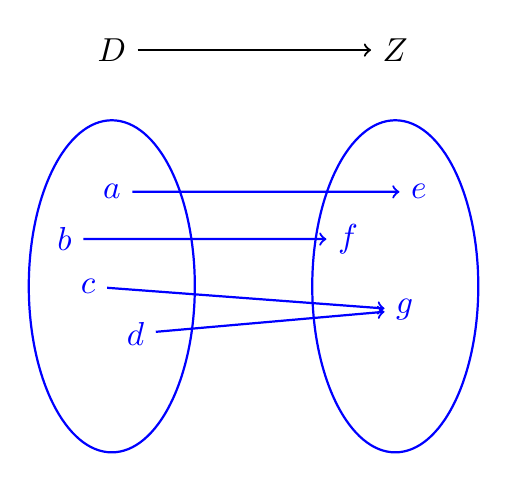
\begin{tikzpicture}[scale=1.2, transform shape]
        \node at (0, 0) (D) {$D$};
        \node at (3, 0) (Z) {$Z$};

        \draw[blue, thick] (0,-2.5) ellipse (2.5em and 5em);
        \draw[blue, thick] (3,-2.5) ellipse (2.5em and 5em);

        \begin{scope}[every path/.style={blue}]
          \node at (0, -1.5) (a) {$a$};
          \node at (-.5, -2) (b) {$b$};
          \node at (-.25, -2.5) (c) {$c$};
          \node at (.25, -3) (d) {$d$};
          \node at (3.25, -1.5) (e) {$e$};
          \node at (2.5, -2) (f) {$f$};
          \node at (3.1, -2.75) (g) {$g$};
        \end{scope}

        \path[->, thick] (D) edge (Z);
        \begin{scope}
          [every path/.style={->, blue, thick}]
          \path (a) edge (e);
          \path (b) edge (f);
          \path (c) edge (g);
          \path (d) edge (g);
        \end{scope}
      \end{tikzpicture}
      \caption{Visualisierung Mathematik Funktion}
    \end{figure}
  \end{frame}

  \subsection{fold}
  \begin{frame}{\inlineracket{fold}}
    \begin{itemize}
      \item Faltungsfunktion berechnet aus einer Menge einen einzelnen Wert
      \begin{itemize}
        \item Typ des Wertes kann gleich dem Typ der Elemente in der Menge sein, muss es nicht
      \end{itemize}
      \item Verknüpft das aktuelle Element mit dem momentanten Zwischenergebnis (Initialwert)
      \item Verwendet dieses Ergebnis als neuen Zwischenergebnis und wiederholt diesen Vorgang
      für jedes Element
      \item \enquote{Die Faltungsfunktion reduziert sozusagen eine Menge auf einen Wert}
      \item \inlineracket{foldl}: Ausführung von links nach rechts.
      \item \inlineracket{foldr}: Ausführung von rechts nach links.
      \item Formaler Aufbau:
      \begin{center}
        \inlineracket{(foldl fct initial elements)}

        \inlineracket{(foldr fct initial elements)}
      \end{center}
    \end{itemize}
  \end{frame}

  \begin{frame}[c]
    \begin{minipage}{.495\textwidth}
      \begin{figure}[ht]
        \centering
        \begin{tikzpicture}[scale=1.15, transform shape]
          \def\f{:}
          \def\offset{0}
          \def\position{left}
          \def\textscale{.7}
          \node at (0 + \offset, 0) (\position a) {\f};
          \node at (-.5 + \offset, -.5) (\position b) {1};
          \node at (.5 + \offset, -.5) (\position c) {\f};

          \node at (0 + \offset, -1) (\position d) {2};
          \node at (1 + \offset, -1) (\position e) {\f};

          \node at (.5 + \offset, -1.5) (\position f) {...};
          \node at (1.5 + \offset, -1.5) (\position g) {\f};

          \node at (1 + \offset, -2) (\position h) {$n$};
          \node[scale=\textscale, transform shape] at (2 + \offset, -2) (\position i) {\textcolor{keywordcolor}{empty}};

          \path (\position a) edge (\position b);
          \path (\position a) edge (\position c);

          \path (\position c) edge (\position d);
          \path (\position c) edge (\position e);

          \path (\position e) edge (\position f);
          \path (\position e) edge (\position g);

          \path (\position g) edge (\position h);
          \path[scale=\textscale, transform shape] (\position g) edge (\position i);

          \def\f{$f$}
          \def\offset{3}
          \def\position{right}
          \node at (2 + \offset, 0) (\position a) {\f};
          \node at (2.5 + \offset, -.5) (\position b) {$n$};
          \node at (1.5 + \offset, -.5) (\position c) {\f};

          \node at (2 + \offset, -1) (\position d) {...};
          \node at (1 + \offset, -1) (\position e) {\f};

          \node at (1.5 + \offset, -1.5) (\position f) {2};
          \node at (.5 + \offset, -1.5) (\position g) {\f};

          \node at (1 + \offset, -2) (\position h) {1};
          \node[scale=\textscale, transform shape] at (0 + \offset, -2) (\position i)
            {\inlineracket{init}};

          \path (\position a) edge (\position b);
          \path (\position a) edge (\position c);

          \path (\position c) edge (\position d);
          \path (\position c) edge (\position e);

          \path (\position e) edge (\position f);
          \path (\position e) edge (\position g);

          \path (\position g) edge (\position h);
          \path (\position g) edge (\position i);

          \path[|->] (.5, 0) edge node[above, align=center, scale=\textscale, transform
          shape] {\inlineracket{foldl f init}} (4.5, 0);
        \end{tikzpicture}
        \caption{Visualisierung von foldl}
      \end{figure}
    \end{minipage}
    \hfill
    \begin{minipage}{.495\textwidth}
      \begin{figure}[ht]
        \centering
        \begin{tikzpicture}[scale=1.15, transform shape]
          \def\f{:}
          \def\offset{0}
          \def\position{left}
          \def\textscale{.7}
          \node at (0 + \offset, 0) (\position a) {\f};
          \node at (-.5 + \offset, -.5) (\position b) {1};
          \node at (.5 + \offset, -.5) (\position c) {\f};

          \node at (0 + \offset, -1) (\position d) {2};
          \node at (1 + \offset, -1) (\position e) {\f};

          \node at (.5 + \offset, -1.5) (\position f) {...};
          \node at (1.5 + \offset, -1.5) (\position g) {\f};

          \node at (1 + \offset, -2) (\position h) {$n$};
          \node[scale=\textscale, transform shape] at (2 + \offset, -2) (\position i) {\textcolor{keywordcolor}{empty}};

          \path (\position a) edge (\position b);
          \path (\position a) edge (\position c);

          \path (\position c) edge (\position d);
          \path (\position c) edge (\position e);

          \path (\position e) edge (\position f);
          \path (\position e) edge (\position g);

          \path (\position g) edge (\position h);
          \path[scale=\textscale, transform shape] (\position g) edge (\position i);

          \def\f{$f$}
          \def\offset{3}
          \def\position{right}
          \node at (0 + \offset, 0) (\position a) {\f};
          \node at (-.5 + \offset, -.5) (\position b) {1};
          \node at (.5 + \offset, -.5) (\position c) {\f};

          \node at (0 + \offset, -1) (\position d) {2};
          \node at (1 + \offset, -1) (\position e) {\f};

          \node at (.5 + \offset, -1.5) (\position f) {...};
          \node at (1.5 + \offset, -1.5) (\position g) {\f};

          \node at (1 + \offset, -2) (\position h) {$n$};
          \node[scale=\textscale, transform shape] at (2 + \offset, -2) (\position i)
            {\inlineracket{init}};

          \path (\position a) edge (\position b);
          \path (\position a) edge (\position c);

          \path (\position c) edge (\position d);
          \path (\position c) edge (\position e);

          \path (\position e) edge (\position f);
          \path (\position e) edge (\position g);

          \path (\position g) edge (\position h);
          \path (\position g) edge (\position i);

          \path[|->] (.5, 0) edge node[above, align=center, scale=\textscale, transform
          shape] {\inlineracket{foldr f init}} (2.5, 0);
        \end{tikzpicture}
        \caption{Visualisierung von foldr}
      \end{figure}
    \end{minipage}
  \end{frame}


  \section{Arbeitsphase}
  \begin{frame}[c]{Arbeitsphase}
    \begin{center}
      \textbf{\LARGE Selbstständiges Arbeiten}
    \end{center}
  \end{frame}
\end{document}
